\chapter{Experimental Details}
\label{app:details}

\section{Models and Data}
The Hubble 1B (16 layers, hidden size 2048) and 8B (36 layers, hidden size 4096) Standard and Perturbed
checkpoints are used as released \citep{allegro2025hubble}. The unlearning target is the birthdate
attribute of $n=44$ forget-set (Unlearn) facts, with $45$ Keep facts as the retain set and an Unseen
held-out set for reference. The four prompt formats are name-only, intro-prefix, full-prefix, and
full-prefix with a suffix; the internal analysis uses full-prefix.

\section{Unlearning Hyperparameters}
\label{app:hp}
Each method is tuned by a small grid search under a keep-as-retain configuration. Selection is
\emph{forget-first}. Among configurations that actually unlearn (Unlearn accuracy at or below chance plus a
heuristic noise margin, set to $0.2$ for a $10$-way infill at chance $0.1$), we choose the one that
maximises Keep accuracy;
configurations that fail to unlearn are penalised by a combined score
$\text{Keep} - \lambda\max(0,\text{Unlearn}-\text{threshold})$ with $\lambda=5$, so they cannot win. The
complete search grid is: NPO learning rate $\in\{2\times10^{-5}, 5\times10^{-5}\}$ and retain weight
$\gamma\in\{0.5,1.0,2.0\}$; GradDiff learning rate $\in\{5\times10^{-6}, 1\times10^{-5}\}$ and
$\gamma\in\{1.0,2.0,4.0\}$; IDK learning rate $\in\{2\times10^{-5}, 5\times10^{-5}\}$; RMU steering
coefficient $\in\{200,500,1000\}$ and $\alpha\in\{50,100\}$. Each configuration is evaluated at checkpoints
every two epochs up to eight, and RMU's intervention layers follow the Hubble configuration ($[5,6,7]$ at
8B, $[3,4,5]$ at 1B). Table~\ref{tab:hp} lists the selected 8B settings. All methods share the same fixed configuration, with the
Keep biographies as the retain set, batch size $1$, 8-bit AdamW, gradient checkpointing, and bfloat16. NPO
uses the reference model as the pre-unlearning checkpoint. The 1B models are re-tuned with the same
procedure and differ mainly in the RMU intervention layers; the selected settings are stored in
\texttt{winners\_hp.json} with the pushed model artifacts. As stated in Section~\ref{sec:m-design}, the same
$44$ forget facts are used for this selection and for the subsequent evaluation, so the study is an analysis
of these trained models rather than an out-of-sample estimate.

\begin{table}[t]
  \centering
  \caption[Selected unlearning hyperparameters (8B)]{Selected unlearning hyperparameters at 8B
  (forget-first grid selection). Shared settings: Keep retain set, batch size $1$, 8-bit AdamW, gradient
  checkpointing, bfloat16.}
  \label{tab:hp}
  \begin{tabular}{lcccl}
    \toprule
    method & learning rate & epochs & retain weight & method-specific \\
    \midrule
    NPO      & $5\times10^{-5}$ & 8 & $\gamma=2.0$ & $\beta=0.1$ \\
    GradDiff & $5\times10^{-6}$ & 8 & $\gamma=4.0$ & n/a \\
    IDK      & $5\times10^{-5}$ & 8 & n/a          & n/a \\
    RMU      & $5\times10^{-5}$ & 2 & n/a          & $\alpha=100$, steering coeff.\ $200$, layers $[5,6,7]$ \\
    \bottomrule
  \end{tabular}
\end{table}

\section{Lens Computation}
The logit lens uses the model's own final normalisation and unembedding, with the two corrections of
Section~\ref{sec:m-lens} (true final logits at the last layer; boundary-safe tokenisation). Ranks are
averaged over the gold sub-token positions and the median is taken over facts. The tuned lens trains one
affine translator per layer (identity-initialised) for $3000$ steps at learning rate $3\times10^{-4}$ with
the KL objective of Equation~\eqref{eq:tunedlens}, reaching a per-layer KL of approximately $0.04$ to $0.06$.
The Jacobian lens is described in Appendix~\ref{app:jacobian}.

\section{Compute}
All model forward passes and unlearning runs were executed on a single NVIDIA A100 GPU per job. The
faithfulness meta-evaluation (Section~\ref{sec:m-metaeval}) is inference-only and completes in a few
minutes; the tuned-lens training and the Jacobian-lens runs are the more expensive components.


\chapter{Deriving and Implementing the Jacobian Lens}
\label{app:jacobian}

\section{First-Order Transport and the Intercept}
Let $g_\ell:\mathbb{R}^d \to \mathbb{R}^{|\mathcal{V}|}$ map the layer-$\ell$ residual state to the final
logits (the remaining blocks followed by the unembedding). For a query state $h$, a first-order Taylor
expansion of $g_\ell$ around a reference state $h_i = h^{(\ell)}(x_i)$ is
\begin{equation}
  g_\ell(h) \;\approx\; g_\ell(h_i) \,+\, J_\ell(x_i)\,(h - h_i),
  \qquad J_\ell(x_i) = \left.\frac{\partial g_\ell}{\partial h}\right|_{h_i}.
\end{equation}
Averaging over $N$ reference inputs $\{x_i\}$ gives the affine readout of Equation~\eqref{eq:jaclens}:
\begin{equation}
  \mathrm{JL}_\ell(h) \;=\; \frac{1}{N}\sum_i \Bigl[g_\ell(h_i) + J_\ell(x_i)(h-h_i)\Bigr]
                    \;=\; A_\ell h + b_\ell,
\end{equation}
with slope $A_\ell = \tfrac{1}{N}\sum_i J_\ell(x_i)$ and intercept $b_\ell = \tfrac{1}{N}\sum_i
\bigl(g_\ell(h_i) - J_\ell(x_i) h_i\bigr)$. The intercept is essential. Without it the readout is only
$A_\ell h$, whose level floats freely per layer and produces a jagged, uninterpretable rank trajectory. Our
first implementation omitted $b_\ell$ and was discarded for this reason; restoring it reduces the
layer-to-layer jaggedness of the trajectory below that of the logit lens itself.

\section{Matrix-Free Jacobian-Vector Products}
Materialising $J_\ell$ (a $|\mathcal{V}|\times d$ matrix) is unnecessary. Each required
Jacobian-vector product $J_\ell(x_i)\,v$ is computed matrix-free by a double-backward. With $y = g_\ell(h)$
and an auxiliary vector $u$, first form $g = \partial\langle y,u\rangle/\partial h$ with a retained graph,
then $J_\ell v = \partial g / \partial u$ evaluated with $\mathrm{grad\_outputs}=v$. This reverse-over-reverse
formulation composes with forward hooks, unlike forward-mode automatic differentiation.

\section{Hook Injection}
To differentiate $g_\ell$ we inject the state $h$ into the model's \emph{own} forward pass via a
forward-pre-hook at layer $\ell$, so that positional encodings and attention masks are exactly the model's.
We verify on every layer that the injection reproduces the true forward pass ($\|\hat y - y\|$ within a
small tolerance), which confirms that the Jacobian-vector products are meaningful and not an artifact of the
injection.

\section{The Diverse-Context Requirement}
A second correction concerns the choice of reference inputs $\{x_i\}$. When the references are the
\emph{same-template} prompts (other birthdate facts), the averaged linear model is locally exact and the
readout trivially reconstructs the query's own output at every layer, producing flat, uninformative rank
curves. Averaging the Jacobian over $24$ reference contexts drawn from a pool of $38$ diverse, generic
sentences (leave-the-query-out) instead yields a generic transport that only decodes the answer once the
state is output-aligned, restoring genuine layer-wise emergence. Both corrections, the intercept and diverse contexts, are needed for a usable readout; with them,
the Jacobian lens reproduces the method taxonomy with a first-order, interventionally-grounded readout
(Figure~\ref{fig:jacobian}) and its
knowledge-versus-prior control (Figure~\ref{fig:jctrl}) confirms that the descent in the readout is driven
by the fact's representation rather than by the intercept prior.

\begin{figure}[t]
  \centering
  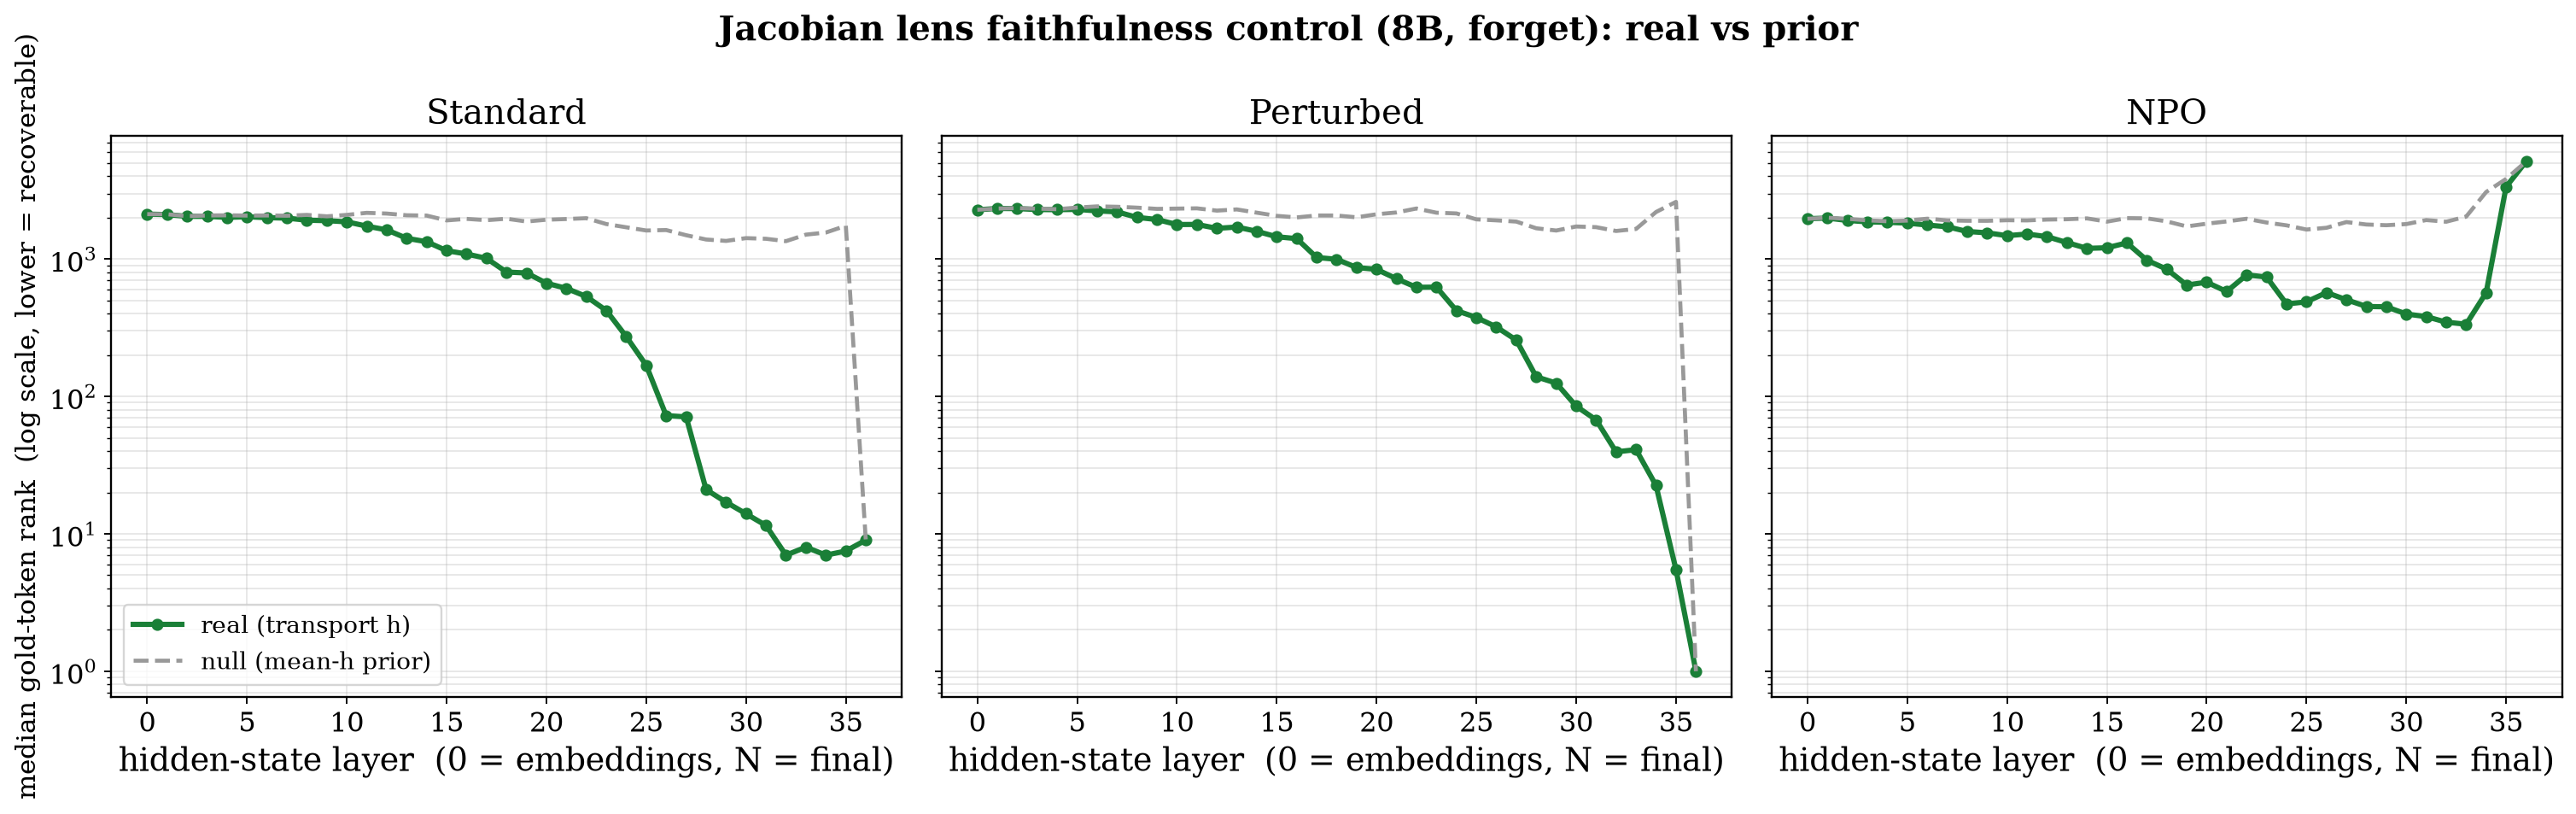
\includegraphics[width=0.95\textwidth]{jlens_affine_control_8b}
  \caption[Jacobian-lens knowledge-versus-prior control (8B)]{Jacobian-lens knowledge-versus-prior control (8B, forget). ``Real'' transports the fact's own
  hidden state; ``null'' transports the fact-agnostic mean. Real falls below null for the knowing model and
  tracks it for the never-knew model, confirming the readout reads knowledge, not the intercept prior.}
  \label{fig:jctrl}
\end{figure}


\chapter{Supplementary Results and Reproducibility}
\label{app:repro}

\section{A Single-Fact Emergence Table}
Figure~\ref{fig:single} shows, for one fact under the knowing model, the top-1 logit-lens prediction at
every layer converging to the correct answer, the layer-by-layer picture of genuine knowledge that the
unlearned models fail to reproduce.

\begin{figure}[t]
  \centering
  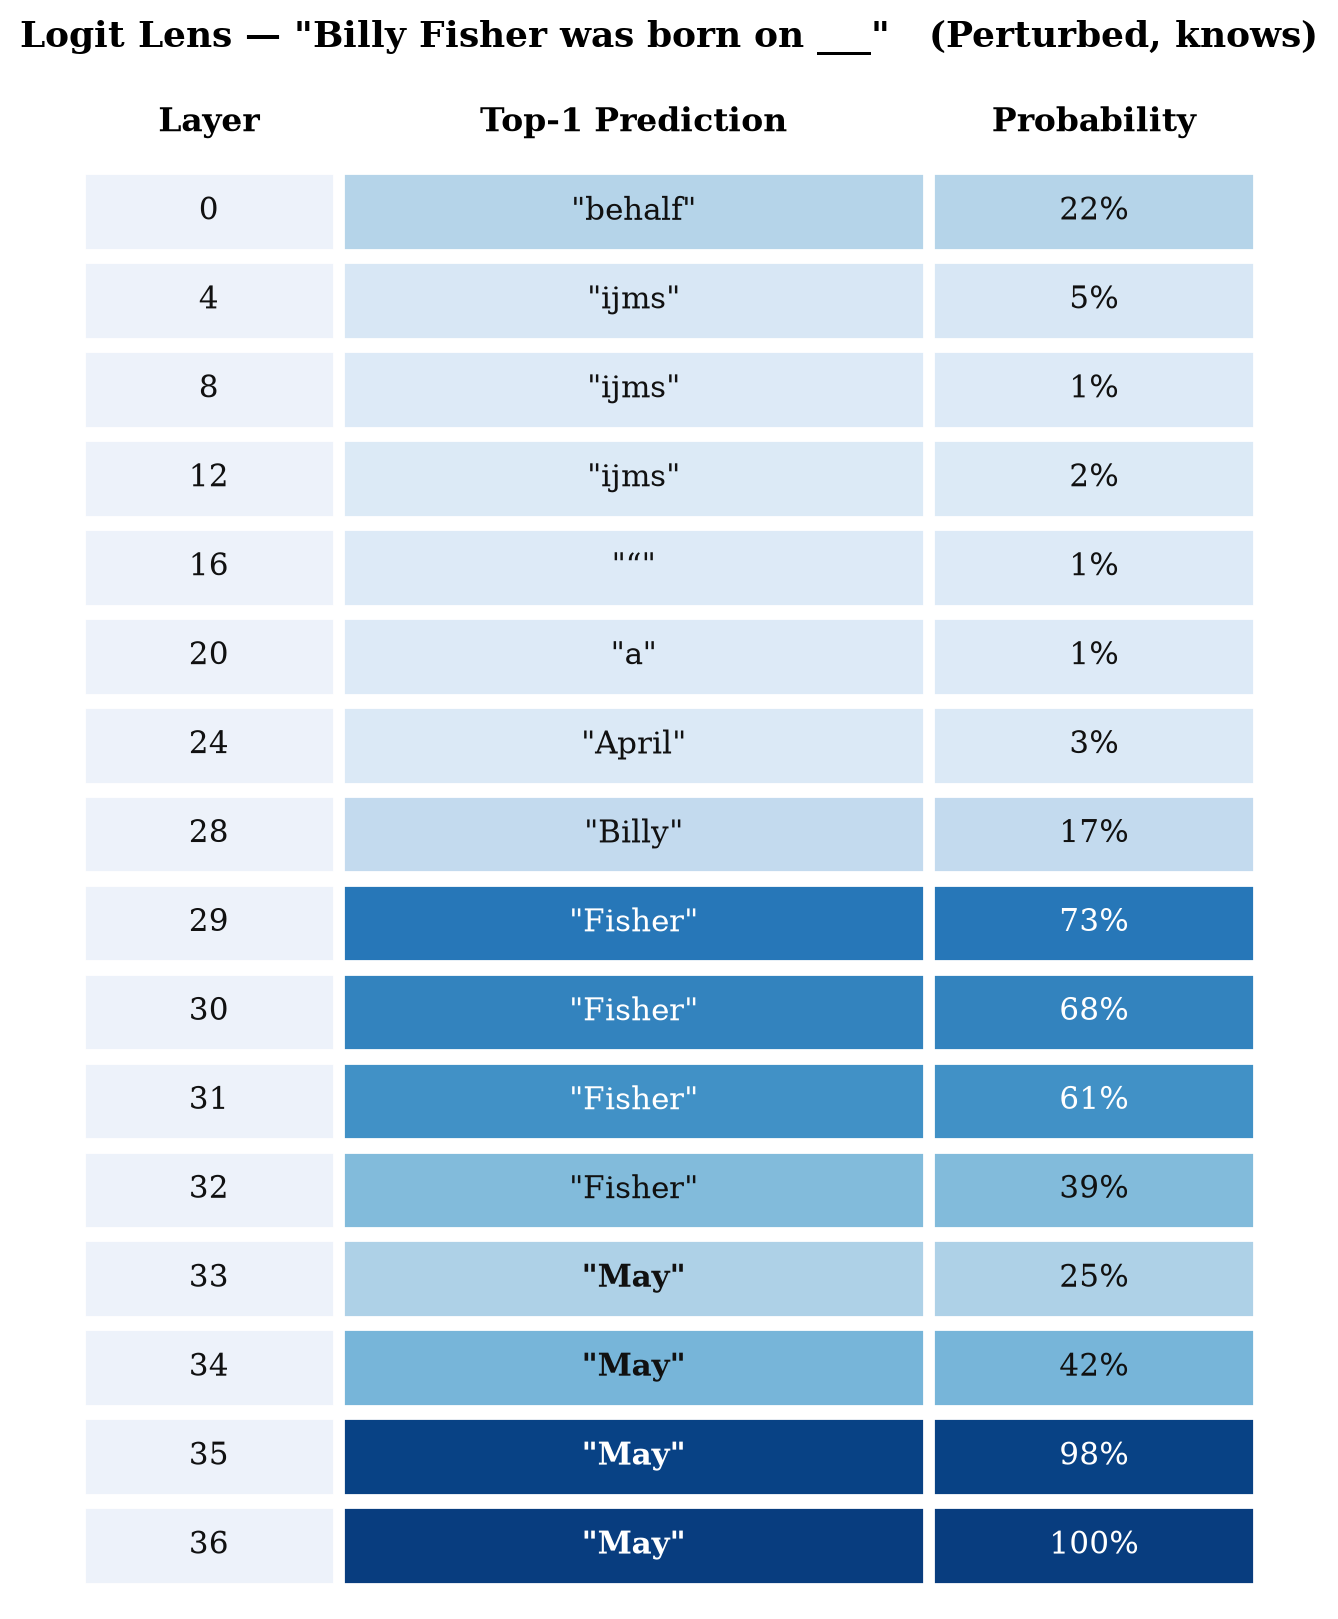
\includegraphics[width=0.55\textwidth]{lenstable_single_0}
  \caption[Single-model logit-lens emergence (8B)]{Single-model logit-lens emergence (Perturbed, 8B). The correct month climbs to the top over the
  final layers, the signature of a fact the model genuinely holds.}
  \label{fig:single}
\end{figure}

\section{Reproducibility}
All experiments are driven by a single code base organised around a scale-invariant harness selected by an
environment variable (1B or 8B). The logit-lens readout, the $D_\text{mech}$ metric, the faithfulness
meta-evaluation, the tuned- and Jacobian-lens computations, and the robustness attacks are each implemented
as a self-contained script with a corresponding batch submission file, using deterministic greedy decoding
and a fixed random seed. The per-instance data behind every table and figure (rank trajectories, metric
cells, effect sizes, attack recoveries) are exported as comma-separated files, and the figures are
regenerated from those files by a single plotting script with a shared style. The code base is archived and
available on request rather than publicly released; the released model and data artifacts, and the software
environment, are identified below.

\begin{description}
  \item[Environment.] Python $3.11$, PyTorch $2.11$ (CUDA $12.8$), Transformers $5.14$; one NVIDIA A100
  80GB per job; random seed $0$; deterministic greedy decoding.
  \item[Hubble models.] \texttt{allegrolab/hubble-\{1b,8b\}-500b\_toks-\{standard,perturbed\}-hf} (revision
  \texttt{step238500}); unlearned checkpoints
  \texttt{Harsh01012/hubble-8b-\{npo,graddiff,idk,rmu\}-unlearned-yago-birthdate}.
  \item[TOFU models.] \texttt{open-unlearning/tofu\_Llama-3.2-\{1B,3B\}-Instruct\_\{full,retain90\}} and
  \texttt{tofu\_Llama-3.1-8B-Instruct\_\{full,retain90\}}.
  \item[Data.] Hubble YAGO birthdate and nationality facts, released with the checkpoints; TOFU
  \texttt{forget10} and \texttt{forget10\_perturbed} from \texttt{locuslab/TOFU}.
\end{description}
